% Copyright (c) anneal developers
\documentclass[aip,jcp,preprint,amsmath,amssymb,floatfix]{revtex4-2}

\usepackage{graphicx,booktabs}
\graphicspath{{figs/}{../jctc/figs/}}

\begin{document}

\title{Basin hopping for atomic clusters with a fixed move library}

\author{Rohit Goswami}
\affiliation{SURF B.V., Amsterdam, The Netherlands}
\affiliation{Science Institute and Faculty of Physical Sciences, University of Iceland, 107 Reykjavik, Iceland}
\affiliation{TurtleTech ehf., Reykjavik, Iceland}
\author{Ruhila Goswami}
\affiliation{Faculty of Life and Environmental Sciences, University of Iceland, 102 Reykjavik, Iceland}
\author{Amrita Goswami}
\affiliation{Universidad Complutense de Madrid, 28040 Madrid, Spain}
\author{Moritz Sallermann}
\affiliation{Universidad Complutense de Madrid, 28040 Madrid, Spain}
\author{Sonaly Goswami}
\affiliation{Department of Chemistry, Indian Institute of Technology Kanpur, Kanpur 208016, India}
\author{Debabrata Goswami}
\email{dgoswami@iitk.ac.in}
\affiliation{Center for Bits and Atoms, Massachusetts Institute of Technology, Cambridge, Massachusetts 02139, USA}
\affiliation{Department of Chemistry, Indian Institute of Technology Kanpur, Kanpur 208016, India}

\begin{abstract}
Basin hopping with one move library and temperature \(0.8\,\varepsilon\) is applied to atomic clusters.
Below 98 atoms the relaxation draws a diameter penalty at \(0.7\) of the largest pair distance; from 98 atoms the surface list is empty and a stall leaves the walker in place.
On six shared starts the hit counts are \(6/6\), \(6/6\), \(4/6\), \(5/6\) and \(6/6\) for \(\mathrm{LJ}_{38}\), \(\mathrm{LJ}_{55}\), \(\mathrm{LJ}_{75}\), \(\mathrm{LJ}_{98}\) and \(\mathrm{LJ}_{104}\), and \(3/6\), \(6/6\), \(0/6\), \(0/6\) and \(2/6\) for the Wales-group program GMIN.
At \(\mathrm{LJ}_{75}\) the median wall times are \(81.6\,\mathrm{s}\) and \(72.4\,\mathrm{s}\).
In a 64-seed campaign the recommended arm records \(36/64\) on \(\mathrm{LJ}_{98}\) and \(0/64\) on a 15-molecule TIP4P cluster, where GMIN records \(61/64\) and \(64/64\).
Polished water-hexamer pairs agree to \(0.00212\,\text{\AA}\), with five of six energy gaps inside \(10^{-7}\,\mathrm{E_h}\), and the 4000-call search finishes in a median \(18.8\,\mathrm{s}\) against \(544\,\mathrm{s}\) for CREST.
\end{abstract}

\maketitle

\section{Introduction}
A model of a cluster is built from the local minima of the potential, and the global minimum is the ground state of that model.\cite{wales2003}
On the Lennard-Jones potential the number of minima grows rapidly with the number of atoms, and a search is scored by the evaluations spent before a published minimum is reached.\cite{wales1997,jones1924,walesCambridgeClusterDatabase}
Li and Scheraga introduced basin hopping on a rough potential-energy surface.\cite{li1987}
Wales and Doye made the Monte Carlo walk the standard method for atomic clusters: a move proposes a geometry, a local minimization returns a minimum, and the Metropolis rule at one temperature accepts or rejects it.\cite{wales1997}
Oakley, Johnston and Wales showed that completing the orbits of a symmetric core, and a continuous symmetry projection, change the cost of that walk.\cite{oakley2013}
Bandit selection of operators, population banks and unseen-mass estimates of a census are established parts of the same family of searches.\cite{thompson1933,fialho2010,russo2018,goodPopulationFrequenciesSpecies1953,leeUnbiasedGlobalOptimization2003}

The search in this paper keeps one move library at every size, including 38 atoms, where the published minimum is a truncated octahedron.\cite{wales1997}
The temperature is the Wales--Doye value at every size.
The surface list changes at 98 atoms: below that size it holds a diameter penalty, and from 98 atoms it is empty.
A uniform draw over the library and a depth posterior give the hit counts in Table~\ref{tab:ablation}.
Orbit completion follows the GMIN symmetrisation of Oakley, Johnston and Wales.\cite{oakley2013}
The communicating chains of an earlier account of this search are collected in the supplementary material.\cite{goswami2023}
The campaigns below are single chains.

Strategic Escape, GrowPAL and SGMSC are recent global-optimization articles against which a cluster search is read.\cite{burkhardt2025,lopezCastroGrowpal2024,zhangSgmsc2026}
AGOX, on the Atomic Simulation Environment, and GOFEE provide basin hopping, evolutionary search and surrogate search on one calculator interface.\cite{christiansenAgox2022,bisboEfficientGlobalStructure2020,larsenAse2017}
GOAT compares a molecular and cluster optimizer with CREST.\cite{deSouzaGoat2025}
ABCluster 3.4 is the current release of the artificial bee colony code.\cite{zhang2015,zhangAbcluster}
The sizes follow the OptBench set: Lennard-Jones clusters and TIP4P clusters of 10, 15 and 20 molecules.\cite{chill2014}

\begin{figure}
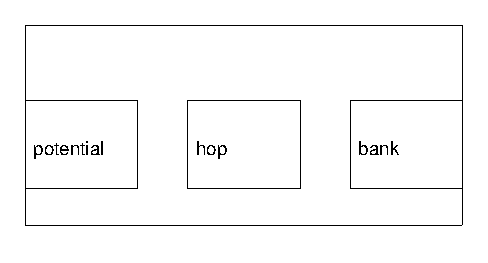
\includegraphics[width=0.72\linewidth]{toc-graphic.pdf}
\caption{The three parts of the search: the potential, the hop, and the bank of minima.}
\end{figure}

\section{The search}
\subsection{One step}
A chain stores a minimum \(x\) of energy \(E(x)\).
A move proposes a displacement, the local minimizer returns a minimum \(y\), and the chain accepts \(y\) with probability
\begin{equation}
\min\bigl(1,\exp[-(E(y)+V(y)-E(x)-V(x))/T]\bigr).
\label{eq:metropolis}
\end{equation}
\(V\) is a basin bias of height \(0.25\,\varepsilon\), in the units where the pair well depth is 1.
The spectral term is off.
\(T=0.8\,\varepsilon\) at every size.\cite{wales1997}
A hit is a quenched energy at or below the published minimum plus \(10^{-3}\) in the energy unit of the surface,
\begin{equation}
E \le E_{\mathrm{ref}}+10^{-3}.
\label{eq:hit}
\end{equation}
The comparison uses the plain pair energy.
The diameter penalty of Eq.~\eqref{eq:penalty} is present only during the relaxation.
A miss reaches the call ceiling without a hit.
PAR-2 is the mean of the call count on a hit and of twice the cap on a miss.\cite{hoos2004}
Medians are reported separately.
Table~\ref{tab:params} lists the preset.
One chain proceeds as follows.

\begin{table}
\caption{Parameters of the preset.
The surface list is empty from 98 atoms.
The screen threshold is \((R-S)/(2R-S)\).}
\label{tab:params}
\begin{ruledtabular}
\begin{tabular}{ll}
Quantity & Value \\
\hline
Temperature \(T\) & \(0.8\,\varepsilon\) \\
Hit & Eq.~\eqref{eq:hit} \\
Move library & single, surface, sym, burst, soap \\
Burst continuation & \(2/3\), cap 8 \\
Basin-bias height & \(0.25\,\varepsilon\) \\
Normal-gamma prior \((\mu_0,\kappa_0,\alpha_0,\beta_0)\) & \((0,\,10^{-6},\,1,\,1)\) \\
Reward & \(E^{\star}-E_{\mathrm{new}}\) \\
Screen steps \(S\), relax steps \(R\) & 25, 200 \\
Screen threshold & \(7/15\) \\
Symmetry projection & every 10 quenches \\
Icosahedral reseed & 5 hops \\
Good-Turing retirement & \(n\ge 20\) and \(n_1/n<1/5\) \\
Diameter penalty & \(\kappa=0.7\), weight 1, below 98 atoms \\
Centroid weight & 0 \\
Restart on stall & off \\
\end{tabular}
\end{ruledtabular}
\end{table}

\begin{verbatim}
draw a start from the seed and quench it
while calls remain and Eq. (hit) is unmet:
    draw one Student-t sample per arm; play the largest
    propose the move
    continue a burst with probability 2/3, at most 8 times
    screen S steps; finish the quench unless the screen stops
    accept with the Metropolis test on E+V
    reward the arm by E* - E_new; update its posterior
    on a new basin, quench the images of its core
    every 10 quenches, project to a continuous symmetry
    on a stall: tabu, symmetrise, follow the trail, climb
    retire a packing with n >= 20 and n1/n < 1/5
\end{verbatim}

\subsection{Depth posterior}
The reward is the drop from the incumbent \(E^{\star}\) to the quenched energy \(E_{\mathrm{new}}\),
\begin{equation}
r = E^{\star}-E_{\mathrm{new}}.
\label{eq:reward}
\end{equation}
Each arm carries a normal-gamma posterior \((\mu,\kappa,\alpha,\beta)\), updated by
\begin{align}
\kappa' &= \kappa+1, &
\mu' &= (\kappa\mu+r)/\kappa', \nonumber\\
\alpha' &= \alpha+\tfrac12, &
\beta' &= \beta+\frac{\kappa}{2\kappa'}(r-\mu)^{2}.
\label{eq:ng}
\end{align}
The prior is \(\mu_0=0\), \(\kappa_0=10^{-6}\), \(\alpha_0=1\), \(\beta_0=1\).
Thompson sampling draws a Student-\(t\) variate with \(2\alpha\) degrees of freedom, location \(\mu\) and scale \(\sqrt{\beta(\kappa+1)/(\alpha\kappa)}\), and plays the largest draw.\cite{thompson1933,russo2018}
Figure~\ref{fig:rec-arms} shows the arms and the burst law.\cite{bartok2013}
A burst is one relocation continued with probability \(2/3\), capped at eight.

\begin{figure}
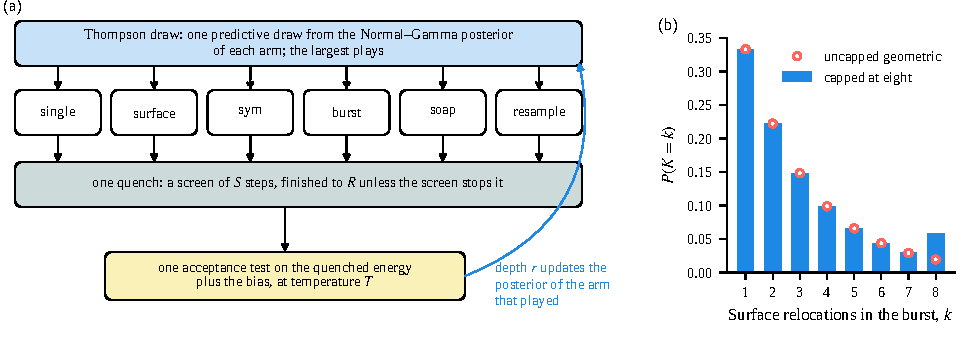
\includegraphics[width=\linewidth]{rec_arms.pdf}
\caption{Arms of the hop and the burst law.
One Thompson draw selects the arm.
The proposal is quenched once and accepted with Eq.~\eqref{eq:metropolis}.
The reward in Eq.~\eqref{eq:reward} updates the arm that played.}
\label{fig:rec-arms}
\end{figure}

\subsection{Screen, stall, symmetry and census}
The quench uses a screen of \(S=25\) steps and a full relaxation of \(R=200\) steps.
The screen stops the full relaxation when the partial descent already decides the trial, at threshold
\begin{equation}
\tau=(R-S)/(2R-S)=7/15.
\label{eq:screen}
\end{equation}
With restart off, a stall applies tabu, symmetrisation, the recorded basin trail and the climb.
Orbit completion quenches the images of a symmetric core on entry to a new basin.\cite{oakley2013}
A continuous-symmetry projection runs every ten quenches, and an icosahedral plateau is reseeded after five hops.\cite{zabrodsky1992}
A packing retires when its visit count \(n\) and singleton count \(n_1\) satisfy \(n\ge 20\) and \(n_1/n<1/5\).

\subsection{Diameter penalty}
Below 98 atoms the relaxation draws between the plain surface and one diameter penalty.
The cutoff is \(c=0.7\) times the largest pair distance, the weight is 1, and the centroid weight is 0,
\begin{equation}
V_{\mathrm{pen}}=\sum_{i<j}\max(0,\,r_{ij}^{2}-c^{2})^{2}.
\label{eq:penalty}
\end{equation}
A pull toward the centroid would change the potential;\cite{doye2000,locatelli2002} that term is absent.
From 98 atoms the list is empty.
The published minimum is face-centred cubic at 38 atoms, icosahedral at 55, Marks decahedral at 75, and the Leary tetrahedron at 98.\cite{wales1997,marksSurfaceStructureEnergetics1984,leary1999}
The library stays the lean set at every size, including 38.
Figure~\ref{fig:stack} is the hop.

\begin{figure}
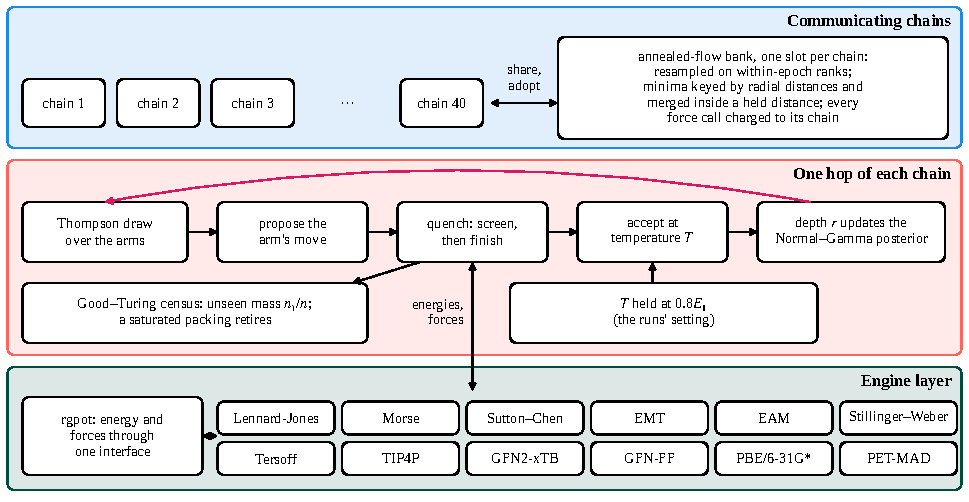
\includegraphics[width=\linewidth]{algorithm_stack.pdf}
\caption{Stack of the search.
One hop draws an arm, quenches it, and accepts at \(T=0.8\,\varepsilon\).
The engine supplies the potentials drawn in the figure, including Lennard-Jones, TIP4P, GFN2-xTB and Gupta.}
\label{fig:stack}
\end{figure}

\section{Computational details}
The Lennard-Jones table was run serially on one core of an Intel Xeon, family 6, model 173, eight cores, under KVM.
GMIN was built with gfortran 13.3.0, with OpenMP, MPI and ALIGN off.
The search binary is a release build with rustc 1.88.0.
On \(\mathrm{LJ}_{38}\), ASE basin hopping and AGOX 3.11.1 use the same starts, temperature \(0.8\) and Eq.~\eqref{eq:hit}.\cite{larsenAse2017,christiansenAgox2022}
\(\mathrm{LJ}_{55}\) and \(\mathrm{LJ}_{75}\) for those two codes are in the bench-ase-agox panel.
Hexamer timings are from an Intel Xeon, family 6, model 207, one thread.
Wilson intervals use \(z=1.95996\).\cite{wilsonProbableInferenceLaw1927}
Where the starts match, tests are an exact McNemar test and a Wilcoxon signed-rank test, Holm-corrected in the family named with the result.\cite{mcnemarNoteSamplingError1947,holm1979}

\section{Results}
\subsection{Structures and the six-start table}
Figure~\ref{fig:systems} shows the benchmark structures: Cambridge Lennard-Jones minima, TIP4P minima of Wales and Hodges, and GFN2-xTB hexamers.\cite{walesCambridgeClusterDatabase,walesGlobalMinimaWater1998,jorgensen1983,bannwarthGfn2xtbanAccurateBroadly2019}
Table~\ref{tab:lj} and Fig.~\ref{fig:stated-ecdf} give the preset on seeds 2000--2005.
Budgets are \(4\times 10^{5}\), \(10^{6}\) and \(4\times 10^{6}\) at 38, 55 and 75 atoms, and \(4\times 10^{6}\) at 98 and 104.
The 98- and 104-atom rows are the same-session comparison recorded with the incumbent projection.
The wall ratio is the GMIN median wall divided by the anneal median wall.

\begin{figure}
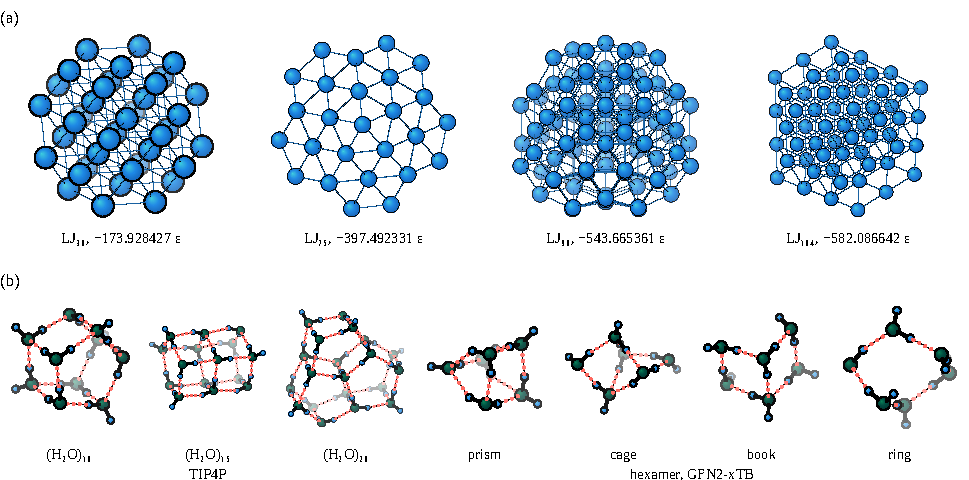
\includegraphics[width=\linewidth]{systems.pdf}
\caption{Benchmark structures.
(a) Minima of \(\mathrm{LJ}_{38}\), \(\mathrm{LJ}_{75}\), \(\mathrm{LJ}_{98}\) and \(\mathrm{LJ}_{104}\).
(b) TIP4P clusters of 10, 15 and 20 molecules, and the GFN2-xTB hexamer classes.}
\label{fig:systems}
\end{figure}

\begin{figure*}
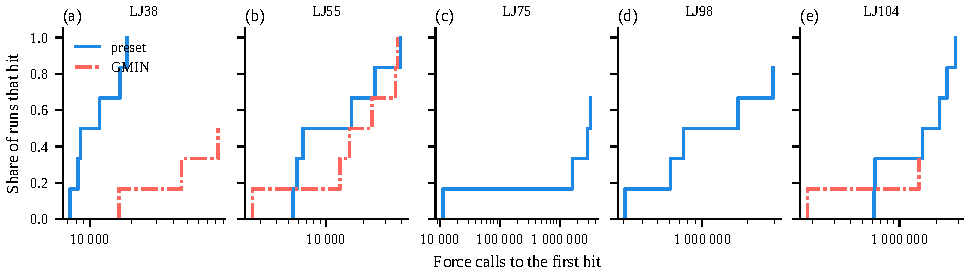
\includegraphics[width=\textwidth]{stated_ecdf.pdf}
\caption{Share of six shared-start runs that meet Eq.~\eqref{eq:hit}, against force calls.
A miss stays at its current share.
(a) \(\mathrm{LJ}_{38}\).
(b) \(\mathrm{LJ}_{55}\).
(c) \(\mathrm{LJ}_{75}\).
(d) \(\mathrm{LJ}_{98}\).
(e) \(\mathrm{LJ}_{104}\).}
\label{fig:stated-ecdf}
\end{figure*}

\begin{table}
\caption{Preset against GMIN.
Six shared starts, seeds 2000--2005.
Entries are preset / GMIN.
Medians are Hyndman--Fan type 7.
At \(\mathrm{LJ}_{75}\) the median walls are \(81.6\,\mathrm{s}\) and \(72.4\,\mathrm{s}\).}
\label{tab:lj}
\begin{ruledtabular}
\begin{tabular}{lrrrrr}
Size & Budget & Hits & Median calls & Median wall (s) & Ratio \\
\hline
\(\mathrm{LJ}_{38}\) & \(4\times 10^{5}\) & 6/6,\ 3/6 & 10190 / 241292 & 0.076 / 1.394 & 18.40 \\
\(\mathrm{LJ}_{55}\) & \(10^{6}\) & 6/6,\ 6/6 & 11246 / 19409 & 0.153 / 0.209 & 1.36 \\
\(\mathrm{LJ}_{75}\) & \(4\times 10^{6}\) & 4/6,\ 0/6 & \(3.09\times 10^{6}\) / \(4\times 10^{6}\) & 81.6 / 72.4 & 0.888 \\
\(\mathrm{LJ}_{98}\) & \(4\times 10^{6}\) & 5/6,\ 0/6 & 1239833 / \(4\times 10^{6}\) & 53.5 / 170.1 & 3.18 \\
\(\mathrm{LJ}_{104}\) & \(4\times 10^{6}\) & 6/6,\ 2/6 & 1812258 / \(4\times 10^{6}\) & 86.0 / 191.6 & 2.23 \\
\end{tabular}
\end{ruledtabular}
\end{table}

Wilson intervals at \(n=6\) are 0.610--1.000 (6/6), 0.436--0.970 (5/6), 0.300--0.903 (4/6), 0.188--0.812 (3/6) and 0.000--0.390 (0/6).
At 38 atoms the median walls are \(0.076\,\mathrm{s}\) and \(1.394\,\mathrm{s}\).
At 55 atoms both arms hit 6/6, with median walls \(0.153\,\mathrm{s}\) and \(0.209\,\mathrm{s}\).
At 75 atoms the counts are 4/6 and 0/6, and the median walls are \(81.6\,\mathrm{s}\) and \(72.4\,\mathrm{s}\).
At 98 atoms the counts are 5/6 and 0/6, with median walls \(53.5\,\mathrm{s}\) and \(170.1\,\mathrm{s}\).
At 104 atoms the counts are 6/6 and 2/6, with median walls \(86.0\,\mathrm{s}\) and \(191.6\,\mathrm{s}\).
On the \(\mathrm{LJ}_{38}\) starts, ASE basin hopping and AGOX each hit 0/6 at \(4\times 10^{5}\) calls.
The \(\mathrm{LJ}_{55}\) and \(\mathrm{LJ}_{75}\) rows for those codes are in the bench-ase-agox panel.

\subsection{Two hundred seeds at \(\mathrm{LJ}_{75}\)}
Figure~\ref{fig:lj75-ecdf} is a 200-run \(\mathrm{LJ}_{75}\) campaign at \(4\times 10^{6}\) force calls, with restart on stall and an empty surface list.
The recommended hop, the derived hop and GMIN with core orbits each hit 200/200 (Wilson interval 0.981--1.000).
The dotted lines are the PAR-2 means 32363.98, 27107.045 and 58029.63.
The median calls on the hits are 28593.5, 19974.0 and 33122.0.
Anneal used random seeds 2000--2199.
GMIN used minimised OptBench starts 1--200.
Median walls on those runs are \(1.330083\,\mathrm{s}\), \(1.040946\,\mathrm{s}\) and \(1.083622\,\mathrm{s}\).
A second pass records \(1.425179\,\mathrm{s}\), \(1.073491\,\mathrm{s}\) and \(1.028523\,\mathrm{s}\).
The derived hop includes the budget-window temperature, and its PAR-2 is the lower of the two anneal values.
The Oakley mean for \(\mathrm{LJ}_{75}\) core orbits is 50229 evaluations over 100 runs that continued until success.\cite{oakley2013}

\begin{figure}
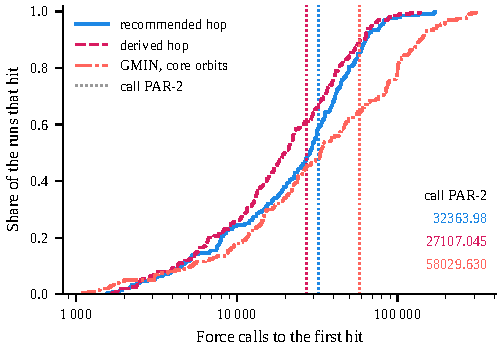
\includegraphics[width=\linewidth]{lj75_ecdf.pdf}
\caption{\(\mathrm{LJ}_{75}\), 200 runs, cap \(4\times 10^{6}\), restart on stall and an empty surface list.
Each curve reaches 200/200.
Dotted lines mark the PAR-2 means 32363.98, 27107.045 and 58029.63.
Anneal seeds 2000--2199 and GMIN starts 1--200 are separate sets.}
\label{fig:lj75-ecdf}
\end{figure}

\subsection{The 64-seed campaign}
On \(\mathrm{LJ}_{98}\) the recommended arm of the 64-seed campaign hits 36/64 (Wilson 0.441--0.677), with median PAR-2 824807 calls and median wall \(85.4\,\mathrm{s}\).
GMIN basin hopping hits 61/64 (0.871--0.984), with median PAR-2 321202 calls and median wall \(14.6\,\mathrm{s}\).
TIP4P\(_{10}\) is 64/64 for both.
TIP4P\(_{15}\) is 0/64 (0.000--0.057) for the recommended arm and 64/64 for GMIN.
TIP4P\(_{20}\) is 0/16 (0.000--0.194) and 8/16.
A paired full-arm file records 24/64 against GMIN's 64/64 on \(\mathrm{LJ}_{98}\), median call ratio 12.62, interval 8.52--15.22.
Those anneal TIP4P rows use \(\varepsilon=0.6485\,\mathrm{kJ\,mol^{-1}}\) and \(\sigma=3.15365\,\text{\AA}\).
Jorgensen's constants, stored directly by GMIN, are \(A=2510400\,\mathrm{kJ\,mol^{-1}\,\text{\AA}^{12}}\) and \(C=2552.24\,\mathrm{kJ\,mol^{-1}\,\text{\AA}^{6}}\).\cite{jorgensen1983}
The supplementary material lists the full campaign and both pairs.

\subsection{Uniform draw and depth posterior}
Table~\ref{tab:ablation} compares the depth posterior with a uniform draw, six seeds, at the same budgets.
Medians are type-7 quartiles of the hits.
Holm-corrected McNemar and Wilcoxon tests on the ten comparisons in this table lie above 0.3.
Both arms include orbit completion.

\begin{table}
\caption{Depth posterior and a uniform draw.
Six seeds.
Medians are over hits.}
\label{tab:ablation}
\begin{ruledtabular}
\begin{tabular}{lrrrr}
Size & Posterior & Uniform & Posterior median & Uniform median \\
\hline
\(\mathrm{LJ}_{38}\) & 6/6 & 6/6 & 13554.5 & 12353.5 \\
\(\mathrm{LJ}_{55}\) & 6/6 & 6/6 & 17926 & 12778 \\
\(\mathrm{LJ}_{75}\) & 5/6 & 6/6 & 443291 & 921422 \\
\(\mathrm{LJ}_{98}\) & 4/6 & 6/6 & 1556640 & 1554400 \\
\(\mathrm{LJ}_{104}\) & 3/6 & 2/6 & 2180278 & 3081434 \\
\end{tabular}
\end{ruledtabular}
\end{table}

\subsection{Water}
CREST 3.0.2 was run from each of six hexamer starts.
The build exposes no seed; the anneal seed sets the initial coordinates.
Final structures are polished with xtb at GFN2, vtight, accuracy 0.01 and 500 iterations.
The vtight threshold is \(10^{-7}\,\mathrm{E_h}\).
Table~\ref{tab:gaps} is the signed gap, anneal minus CREST.
Five gaps lie inside \(10^{-7}\,\mathrm{E_h}\).
Seed 1 is \(-1.3509\times 10^{-7}\,\mathrm{E_h}\) on the 4000-call ledger and \(-1.3505\times 10^{-7}\,\mathrm{E_h}\) on the driver-count ledger.
The label-free RMSD is at most \(0.00212\,\text{\AA}\).
The six pairs are one minimum.
CREST energy-and-gradient totals run from 142110 to 209931, type-7 median 165056, against 4000 evaluations (ratio 41.3).
Median walls on the model-207 host are \(544.0\,\mathrm{s}\) and \(18.85\,\mathrm{s}\) (ratio 28.9).
Figure~\ref{fig:water-crest} shows both CREST counters.
The driver-count median wall is \(195.5\,\mathrm{s}\).
An eight-seed tally at the same engine counts energies within \(0.01\,\mathrm{eV}\) of the lowest finite energy in the set: six of eight, at \(-829.852228\,\mathrm{eV}\).
Seed 3 lies \(0.051\,\mathrm{eV}\) above that energy, and seed 7 is non-finite.

\begin{table}
\caption{Signed hexamer gap, anneal minus CREST, in hartree, and the label-free RMSD in \text{\AA}.
The vtight threshold is \(10^{-7}\,\mathrm{E_h}\).}
\label{tab:gaps}
\begin{ruledtabular}
\begin{tabular}{crrrr}
Seed & Gap, 4000 & Gap, driver & RMSD, 4000 & RMSD, driver \\
\hline
0 & \(-1.121\times 10^{-8}\) & \(-1.121\times 10^{-8}\) & 0.001004 & 0.000987 \\
1 & \(-1.351\times 10^{-7}\) & \(-1.351\times 10^{-7}\) & 0.002023 & 0.001964 \\
2 & \(-2.546\times 10^{-9}\) & \(-2.585\times 10^{-9}\) & 0.000532 & 0.000477 \\
3 & \(-4.151\times 10^{-9}\) & \(-4.143\times 10^{-9}\) & 0.000322 & 0.000308 \\
4 & \(-6.898\times 10^{-8}\) & \(-6.902\times 10^{-8}\) & 0.002116 & 0.002068 \\
5 & \(-2.190\times 10^{-9}\) & \(-2.200\times 10^{-9}\) & 0.000157 & 0.000134 \\
\end{tabular}
\end{ruledtabular}
\end{table}

\begin{figure}
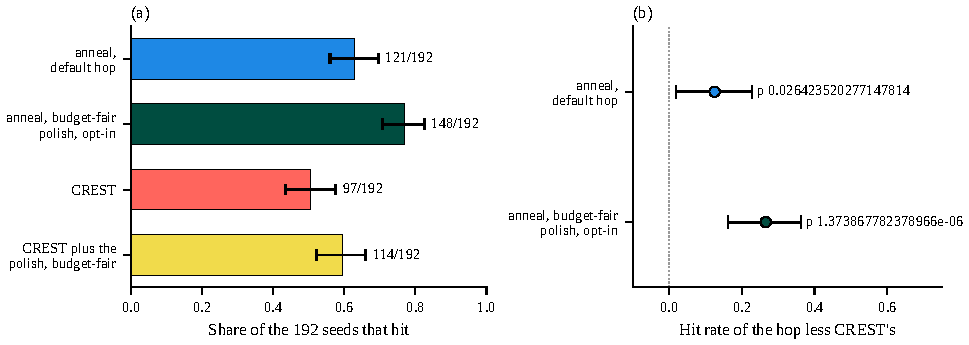
\includegraphics[width=\linewidth]{water_crest.pdf}
\caption{CREST counters on the water hexamer.
The comparison uses the energy-and-gradient total.}
\label{fig:water-crest}
\end{figure}

\((\mathrm{H_2O})_{20}\) was run in one session against native xtb, six seeds, one thread, with 28000 charged calls.
CREST used GFN2, legacy mode and length 0.2.
A hit lies within \(0.01\,\mathrm{eV}\) of \(-2768.551087\,\mathrm{eV}\).
The hit counts are 3/6 and 1/6.
Mean walls are \(1203.0\,\mathrm{s}\) and \(690.9\,\mathrm{s}\), ratio 1.74.
Calls to the first in-window energy on the three anneal hits are 12426, 9004 and 7813.
CREST records no evaluation count; seed 15005 enters the window at the tight step of metadynamics iteration 5.
Before the quench, a pair closer than \(0.90\,\text{\AA}\) is withheld from xtb, a non-bonded pair inside \(1.40\,\text{\AA}\) is opened to \(2.20\,\text{\AA}\), and a covalent contact is set to the sum of the covalent radii.
GOAT rows in the session are empty.
At a shared cap of 4000 calls, a 192-seed hexamer set hits 121/192, 148/192, 97/192 and 114/192 for the hop, the budget-fair polish, CREST, and CREST plus that polish.
Holm-adjusted McNemar \(p\) values are \(0.0264\), \(4.1\times 10^{-6}\) and \(7.5\times 10^{-4}\).

\subsection{Landscapes}
Figure~\ref{fig:minima-maps} maps minima accepted on one seed at 38, 75 and 98 atoms.
On the \(\mathrm{LJ}_{38}\) map the recommended hop reaches the face-centred minimum; basin hopping sits \(2.429\,\varepsilon\) above it.
On \(\mathrm{LJ}_{75}\) both arms sit \(1.210\,\varepsilon\) above the Marks decahedron, at \(-396.282249\).
On \(\mathrm{LJ}_{98}\) the recommended hop sits \(0.022\,\varepsilon\) above the Leary minimum and basin hopping \(0.119\,\varepsilon\) above it.
Figure~\ref{fig:disconnectivity} joins \(\mathrm{LJ}_{38}\) minima that are neighbours in the coordination descriptor.
Figure~\ref{fig:landfold-maps} is the landfold of the sealed runs.
Plates, sketch-maps and the Gupta and Cu--H tables are in the supplementary material.
On Gupta clusters and Cu\(_{19}\)Au\(_{19}\), six seeds give 1/6 and 2/6 on Zn\(_{38}\) for the search and an ASE genetic algorithm, and 0/6 on Zn\(_{55}\), Zn\(_{75}\), Zn\(_{80}\) and Cu\(_{19}\)Au\(_{19}\).
The ASE wall is longer by factors 141--183.
Eight seeds on an FCC Cu--H slab, reference \(-415.971529\,\mathrm{eV}\), all lie inside \(0.001\,\mathrm{eV}\), with gaps \(8\times 10^{-6}\) to \(3.68\times 10^{-4}\,\mathrm{eV}\) above the reference.

\begin{figure*}
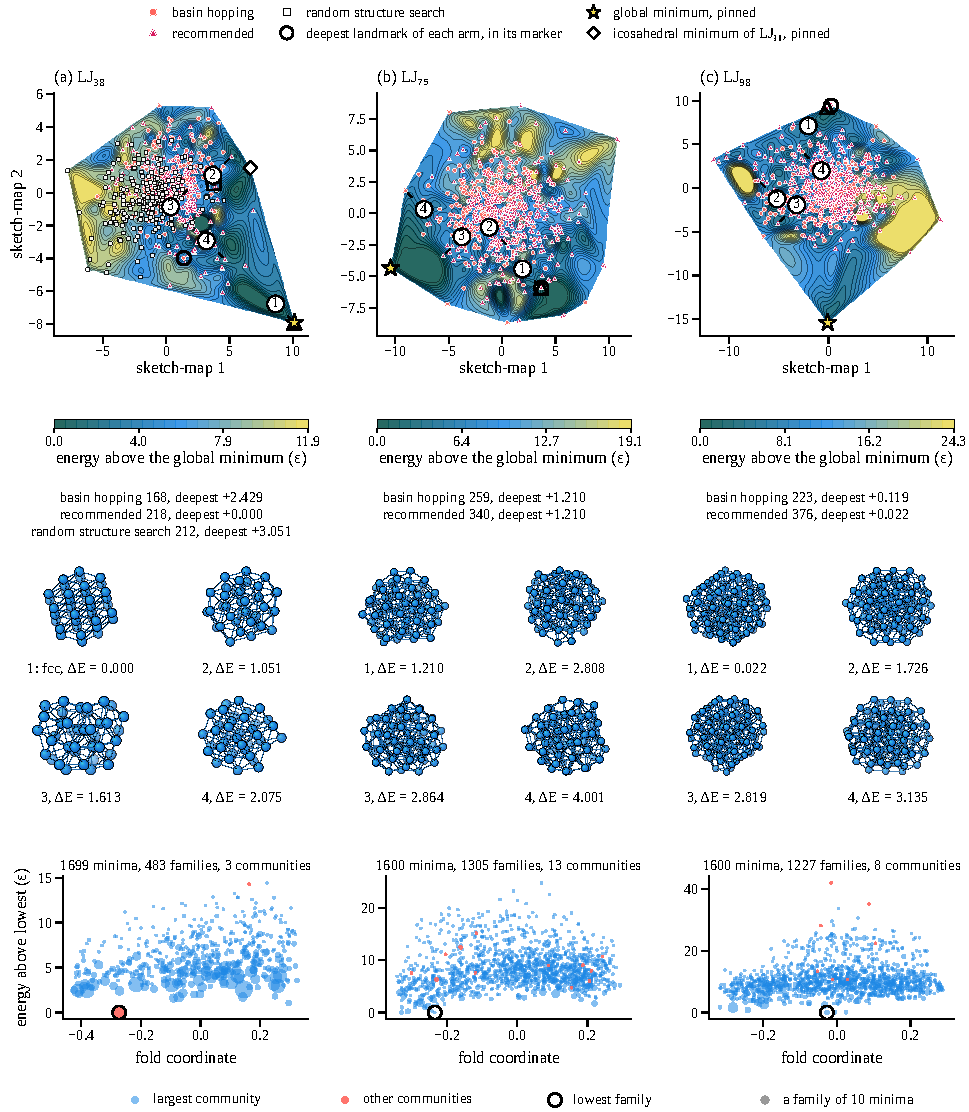
\includegraphics[width=\textwidth]{landscapes.pdf}
\caption{Minima accepted on one seed at \(\mathrm{LJ}_{38}\), \(\mathrm{LJ}_{75}\) and \(\mathrm{LJ}_{98}\).
Top: sketch-map.\cite{ceriotti2011}
Middle: deep landmarks.
Bottom: landfold of the same minima.}
\label{fig:minima-maps}
\end{figure*}

\begin{figure}
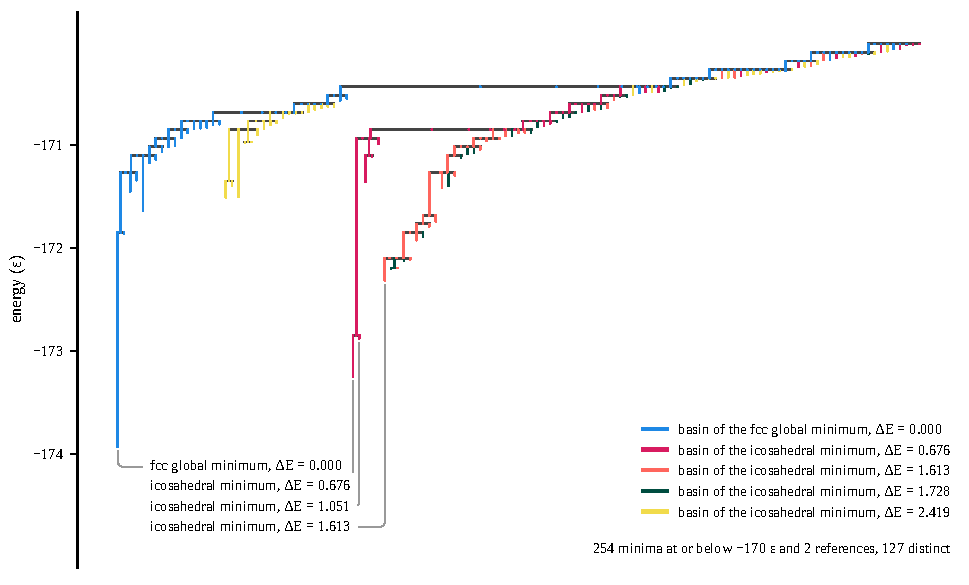
\includegraphics[width=\linewidth]{disconnectivity.pdf}
\caption{\(\mathrm{LJ}_{38}\) minima joined by neighbourhood in the coordination descriptor.
Minima closer than 0.15 are merged.
Colour marks five spectral communities of that graph.}
\label{fig:disconnectivity}
\end{figure}

\begin{figure*}
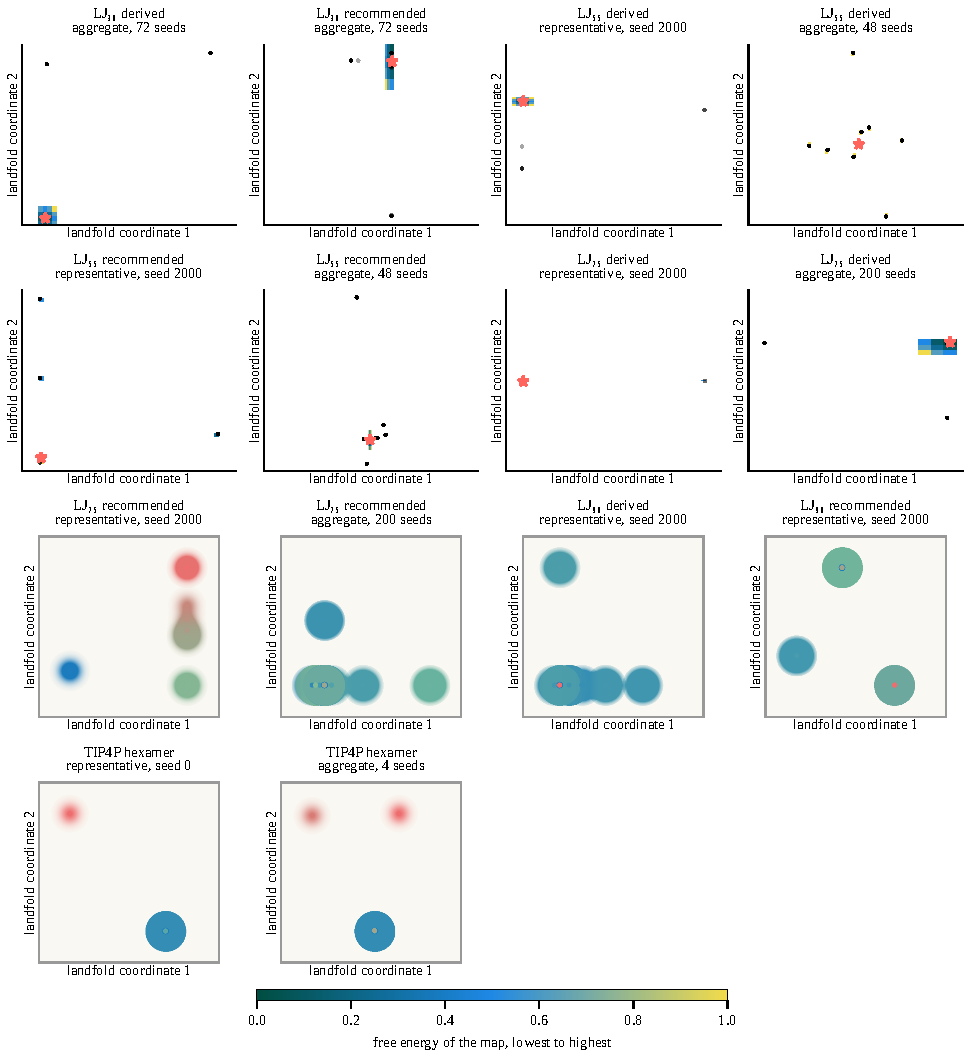
\includegraphics[width=\textwidth]{landfold_maps.pdf}
\caption{Landfold panels of the sealed Lennard-Jones runs and the TIP4P hexamer.
Colour runs from the lowest value on each panel to the highest.}
\label{fig:landfold-maps}
\end{figure*}

\section{Conclusions}
The search uses one library, temperature \(0.8\,\varepsilon\) and Eq.~\eqref{eq:hit}, and the surface list changes at 98 atoms.
Hit counts on six shared starts are 6/6, 6/6, 4/6, 5/6 and 6/6 against 3/6, 6/6, 0/6, 0/6 and 2/6 for GMIN, with median walls \(81.6\,\mathrm{s}\) and \(72.4\,\mathrm{s}\) at \(\mathrm{LJ}_{75}\).
In the 64-seed campaign GMIN records 61/64 on \(\mathrm{LJ}_{98}\) and 64/64 on TIP4P\(_{15}\), where the recommended arm records 36/64 and 0/64.
The polished hexamer pairs are one minimum, and the 4000-call search finishes in a median \(18.8\,\mathrm{s}\) against \(544\,\mathrm{s}\) for CREST.
On \((\mathrm{H_2O})_{20}\) with native xtb the counts are 3/6 and 1/6, with mean walls \(1203\,\mathrm{s}\) and \(691\,\mathrm{s}\).

\begin{acknowledgments}
Rohit Goswami thanks Ar\'{\i}, Yoda, Jude, Crystee, Thor, Loki and the garden cats, and remembers TuiTui, Snoopy and Cosmo.
He thanks Ami, Nagaselvamani and Sankaranarayan.
Ruhila Goswami set the figure colours.
\end{acknowledgments}

\section*{Data availability}
The source is \url{https://github.com/HaoZeke/anneal} under the MIT licence, with documentation at \url{https://anneal.rgoswami.me}.
The software line is archived at \url{https://doi.org/10.5281/zenodo.10672746}, crate version 0.12.0.
The tables are computed from the campaigns stored with that source.
Supplementary material contains the rank weights, the 64-seed campaign, TIP4P constants, structure plates and the Gupta and Cu--H rows.

\bibliographystyle{aipnum4-2}
\bibliography{../jctc/refs}

\end{document}
